\documentclass[a4paper]{article}
\usepackage[utf8]{inputenc}
\usepackage{float}
\usepackage{pdfpages}
\usepackage{textcomp}
\usepackage{indentfirst}

\setlength{\parskip}{1em}

% Colour Management
\usepackage{color}

% Multi-Line Comments
\usepackage{comment}

% Customisable Sections
\usepackage{titlesec}

% Images and Captions
\usepackage{graphicx}
\usepackage{subcaption}
\usepackage{wrapfig}
\graphicspath{{./images/}}
\usepackage{fancyhdr} 


% Bibliography
\usepackage[nottoc]{tocbibind}
\usepackage[
    backend=biber,
    style=ieee]{biblatex}

\addbibresource{report_citations.bib} %Imports bibliography file



% Tables
\usepackage{xcolor}
\usepackage{array}
\newcolumntype{L}{>{\raggedright\arraybackslash}m{0.9\linewidth}}

% Contents Page
\usepackage{hyperref}

% Appendices
\usepackage[toc,page]{appendix}

% Bold Maths Symbols
\usepackage{bm}

% Allowing lower levels of Contents Page
\setcounter{tocdepth}{4}
\setcounter{secnumdepth}{5}

% Make margins smaller, feel free to change
\usepackage{geometry}
\geometry{
textwidth=426pt
}





\title{Engineering Design Project}
\author{Georgio Chaimali \and 
        Dimitrios Georgakopoulos \and 
        Edvard J. Skaarberg Holen \and 
        Hyunjoon Jeon \and 
        Josiah Mendes \and 
        Raghav Viswakumar}
\begin{document} 
\begin{titlepage}
    \setlength{\headheight}{66.89pt}
    \thispagestyle{fancy}
    \renewcommand{\headrulewidth}{0pt}
    \renewcommand{\footrulewidth}{0pt}
    \lhead{
\includegraphics[scale=0.1]{logo.png}}
    \cfoot{} % this is to remove the page number
    \hbox{}\vfill
    \begin{center} 
	    {\scshape\LARGE Imperial College London  \par}
	    \vspace{1cm}
        {\scshape\Large Second Year Design Project\par}
        \vspace{0.25cm}
        {\scshape\Large ELEC50003/ELEC50008\par}
        \vspace{1.5cm}
        {\huge\bfseries The MARS Rover\par}
        \vspace{2cm}
        {\Large\itshape Group 1\par}
        \vfill
        \begin{flushright}
            \textsl{ \large
            Georgio Chaimali \\ 
            Dimitrios Georgakopoulos \\ 
            Edvard J. Skaarberg Holen \\ 
            Hyunjoon Jeon \\ 
            Josiah Mendes \\ 
            Raghav Viswakumar
            }
        \end{flushright}
        \vfill

        % Bottom of the page
        {\large Word Count: XXXX Words \\ \today\par}
    \end{center}
\end{titlepage}
 

\tableofcontents

\newpage

\section{Overview}

\section{Systems}

\subsection{Control}
\subsection{Comms}

\subsection{Vision}
\begin{abstract}
    The purpose of the Vision module is threefold:
    1. Capture data from camera module;
    2. Detect objects of interest within the current view and 
        send their location to the Control module; and
    3. Send image data to Control for streaming to Command. 
\end{abstract}

\subsubsection{Hardware Organisation}

The Vision module comprises of two main hardware elements: 
    the Terasic DE10-Lite, a cost-effective Intel MAX 10 based FPGA board 
    \cite{TerasicDE10Web} 
    and the Terasic D8M-GPIO camera package \cite{TerasicD8MWeb}
that interfaces with the FPGA through the onboard GPIO connectors. 

These hardware choices were made by the project organisers, 
but are also sufficient and capable of carrying out the tasks at hand. 
As the FPGA's hardware is configurable, 
it is more flexible than other embedded systems 
that are limited to a general purpose processor,and 
is also able to handle both streaming and processing of high resolution images
without significant compromises on framerate or data speed 
through the use of concurrent operations and dedicated blocks 
for signal processing applications like multiplication.
This particular FPGA is also equipped with a 4-bit VGA output 
which is useful for debugging object detection live, 
and also has a connector for an Arduino Uno R3 shield, \cite{TerasicDE10Web} 
which can be used to interface with the ESP32 used for control.  

In order to perform general purpose operations like
    to configure camera settings
    and to provide a debugging interface,
a Nios II soft core was instantiated on the FPGA. 
Alternatively, to implement a more advanced image processing algorithm
or to reduce other hardware components in the system like the multiple Arduinos, 
a FPGA with a hard core, 
known as a FPGA System-On-Chip (FPGA SoC) \cite{FPGASoC} could be used, 
which would provide both the advantages of having reconfigurable hardware 
and a more capable general purpose processor. 

\subsubsection{Image Capture Processing Stream}

The image capture and buffering is based on a starter project provided
by Terasic Inc for the D8M Camera module that was modified by Ed Stott 
\cite{EEE2Rover}. 



\subsection{Drive}

% Start of energy subsection
\subsection{Energy}
\begin{abstract}
    
\end{abstract}

\subsubsection{Characterising Components}

\subsubsection{PV Array Configuration}
    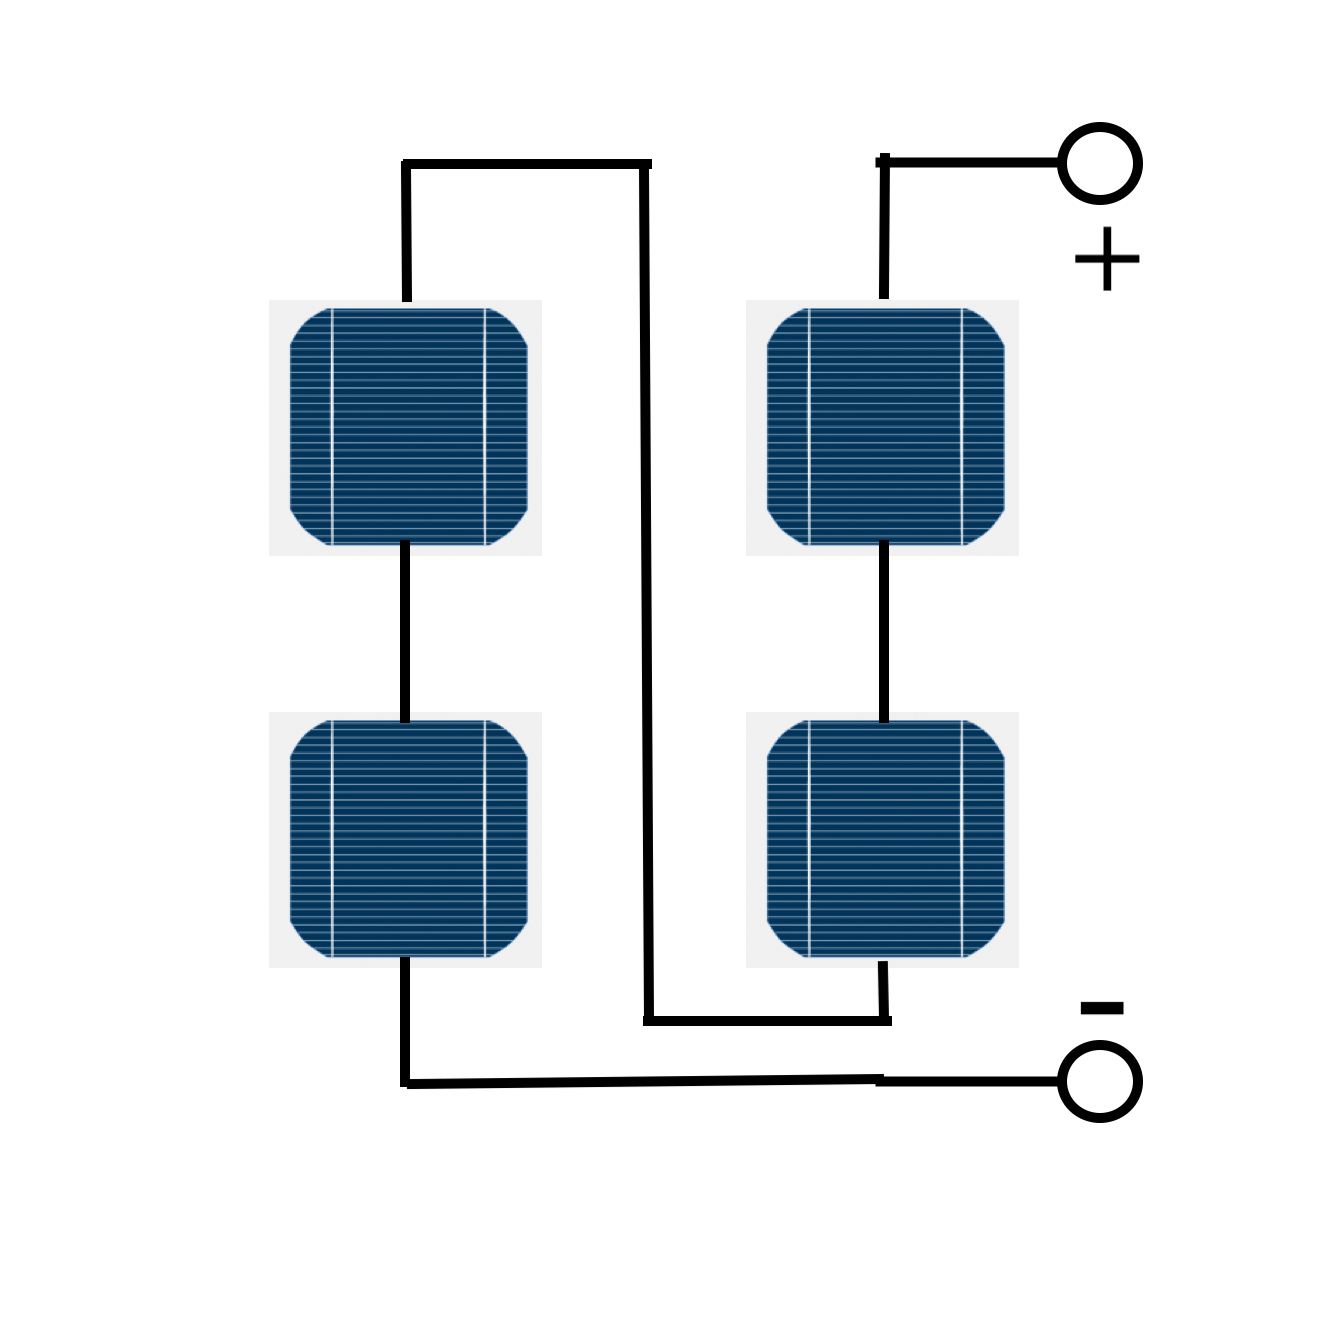
\includegraphics[scale=0.3]{Series(S)}
\subsubsection{Battery Configuration}

\subsubsection{SMPS Configuration}

\subsubsection{Maximum Power Point Tracking}

\subsubsection{Charging Algorithm}

\subsubsection{Discharging Algorithm}

\subsubsection{Safety Mechanisms}

\subsubsection{State of Charge}

\subsubsection{State of Health}

\subsubsection{Communicating with Other Modules}
Though it is not necessary to fully integrate the energy module with the rest of the rover, other submodules, specifically command, needs access data such as the battery SOH and SOC. For communicating with other modules the Arduino shield has a set of UART ports. However, as group members were not in the same location it was not possible to physically connect the energy module to the rover, which is necessary to use UART. As such, an alternative approach was employed. First the Arduino was connected to a computer via USB. On the computer a Python script was run [8]. At the start the Python script establishes a connection to a server created by running a similar script on the command module [9]. After a connection has been established the Python script starts reading the serial data coming from the Arduino and transmits it using TCP to the command module. Each message coming from the Arduino is in CSV form where the first entry is the message ID, which allows the command script to decode what type of data is being sent. 

% End of energy subsection

\subsection{Integration}

% Do not worry George I will take charge in writing this subsubsection -Edvard
\subsubsection{Integrating the Energy Module}

\section{Evaluation and Conclusion}

\section{Intellectual Property}

\newpage

\printbibliography[
heading=bibintoc,
title={References}
]


\begin{figure}[H]
\centering

\includegraphics[scale=0.18]{logo.png}
\caption{Sample Figure}
\label{fig:image1}
\end{figure}

Sample Reference\cite{einstein}


\begin{appendices}
\chapter{Some Appendix}
The contents...
\end{appendices}

\end{document}